\documentclass[conference,letterpaper]{IEEEtran}
\usepackage[T1]{fontenc}
\usepackage[utf8]{inputenc}
\usepackage{microtype}
\usepackage{balance}
\usepackage{amsmath,booktabs,tabularx,array}
\usepackage{graphicx,tikz}
\usetikzlibrary{arrows.meta,positioning,shapes.geometric}
\usepackage{enumitem}
\usepackage[hidelinks,breaklinks]{hyperref}
\hypersetup{pdftitle={Parcel Guard: Design and Evaluation of a Simulated Package Delivery Security Box},pdfauthor={Joshua Guico, Joe Jimenez, Brandon Lopez},pdfsubject={CS 5650 final project report},pdfkeywords={Webots, lockbox, access control, fault recovery, software engineering}}
\urlstyle{same}
\setlength{\emergencystretch}{2em}
\setlength{\parindent}{1em}
\setlength{\parskip}{0pt}
\setlist{nosep,leftmargin=*}
\setcounter{tocdepth}{2}
\renewcommand{\arraystretch}{1.15}
\pagestyle{plain}
\widowpenalty=10000
\clubpenalty=10000
\newcolumntype{Y}{>{\raggedright\arraybackslash}X}
\newcommand{\code}[1]{\texttt{\small #1}}
% The build script refreshes only the following evidence values from saved reports.
\newcommand{\Presence}{50/50}
\newcommand{\MacroF}{1.00}
\newcommand{\FalseAlarms}{0}
\newcommand{\Cycles}{100}
\newcommand{\LatencyCount}{30}
\newcommand{\Recovered}{100}
\newcommand{\Unauthorized}{0}
\newcommand{\BaselineF}{0.10}
\newcommand{\ObserverDelay}{0.224}
\newcommand{\Regressions}{38}
\newcommand{\ReportVersion}{2.4.0}
\newcommand{\BuildDate}{October 17, 2026}
\begin{document}
\onecolumn
\thispagestyle{empty}
\vspace*{0.85in}
\begin{center}
{\fontsize{20}{24}\selectfont\bfseries Package Delivery Security Box\par}
\vspace{0.18in}
{\fontsize{16}{20}\selectfont Webots Simulation for Secure Package Delivery\par}
\vspace{0.55in}
{\fontsize{14}{18}\selectfont CS 5650 Group Project: Final Report\par}
\vspace{0.12in}
{\fontsize{14}{17}\selectfont Master of Science in Computer Science\par
Department of Computer Science\par
California State University, Los Angeles\par}
\vspace{0.5in}
{\fontsize{12}{15}\selectfont
\begin{tabular}{@{}ll@{}}
\textbf{Team Members:} & Joshua Guico\\
 & Joe Jimenez\\
 & Brandon Lopez\\[0.18in]
\textbf{Instructor:} & Dr. Jung Soo Lim\\
\textbf{Semester:} & Fall 2026
\end{tabular}\par}
\vfill
{\large \BuildDate\par}
\end{center}
\clearpage
\thispagestyle{empty}
\tableofcontents
\clearpage
\twocolumn
\title{Parcel Guard: Design and Evaluation of a Webots\\Package Delivery Security Box}
\author{\IEEEauthorblockN{Joshua Guico, Joe Jimenez, and Brandon Lopez}
\IEEEauthorblockA{M.S. Computer Science\\Department of Computer Science\\California State University, Los Angeles\\Fall 2026}}
\maketitle
\thispagestyle{plain}
\begin{abstract}
This project implements a package delivery security box in Webots. A courier uses temporary access to deposit a parcel, and the owner retrieves it later. Virtual sensors and a Python controller detect parcel changes, check door and bolt positions, and record access, fault, and tamper events. A local interface displays status, while an acknowledged message queue retains events during simulated outages. The final tests produced \Presence\ correct presence decisions, four-class macro F1 of \MacroF\ across 60 sequences, and \FalseAlarms\ false tamper alarms among 45 non-tamper sequences. All \Cycles\ motor cycles completed, all \Recovered\ offline alerts were recovered without duplicate processing, and 30 invalid access attempts caused \Unauthorized\ unauthorized unlocks. These results apply to the generated simulation scenarios. The report describes the implementation, test method, corrected failures, and limits of the model.
\end{abstract}
\begin{IEEEkeywords}
Webots, Python, package delivery, access control, simulation, security box, event logging.
\end{IEEEkeywords}
\section{Introduction}
\label{sec:intro}
Packages can arrive when no one is home. Our project models a delivery box that gives a courier temporary access, detects a parcel placed inside, checks that the door and bolt have closed, and records what happened. The owner can later open the box and retrieve the parcel. We call the completed simulation Parcel Guard.

\subsection{Problem and Project Scope}
A delivery notification does not by itself confirm that a parcel remains inside a particular container or that the container has locked. The controller checks those conditions from virtual sensor readings. It also handles incorrect access codes, unexplained movement, blocked actuators, and loss of the simulated message link.

The proposal defines one box, one parcel at a time, and a local simulation \cite{proposal}. The implementation includes an enclosure and parcel model, Python controllers, a local Webots Robot Window, test fixtures, exported measurements, and demonstrations. It requires no purchased hardware or cloud service. This is a CS 5650 course project under Dr. Jung Soo Lim; the proposal names no external sponsor or liaison. The final assignment calls for a paper and class presentation and assesses design, implementation, evaluation, and communication \cite{rubric}.

\subsection{Design Goals}
The goals remain those set out in the proposal: detect delivery and retrieval, restrict access by role, confirm the latch position, record suspected tampering, and recover queued events after an outage. Security status requires measured closure and bolt extension. Scenario generation is separate from event detection so predictions can be compared against independently assigned labels. Loss of the simulated message link leaves local sensing and control running, with events retained until acknowledgment.

\subsection{Team Responsibilities and Development Process}
Table~\ref{tab:team} follows the responsibility allocation in the written proposal. The roles describe the planned division of work; integration, results review, and presentation preparation are shared.
\begin{table*}[t]
\centering\small
\caption{Team responsibilities from the written proposal.}\label{tab:team}
\begin{tabularx}{\textwidth}{@{}l>{\raggedright\arraybackslash}p{.25\textwidth}Y@{}}\toprule
Team member & Assigned role & Project responsibilities \\\midrule
Joe Jimenez & Simulation \& Modeling Lead & Build the Webots enclosure, parcel, door, and latch; configure sensors; create delivery, retrieval, and tamper scenarios; verify simulated component behavior.\\
Joshua Guico & Project \& Integration Lead & Organize tasks, deadlines, and team communication; combine the simulation, controller, interface, and tests; coordinate the demonstration, presentation, and report.\\
Brandon Lopez & Controller, Interface \& Testing Lead & Develop the Python controller and access rules, build the local interface, automate scenarios, collect results, and troubleshoot access and recovery behavior.\\\bottomrule
\end{tabularx}
\end{table*}

Development proceeded through world and sensor modeling, controller/interface integration, and evaluation. The repository mirrors these boundaries. Pure policy tests run without Webots; simulation tests then exercise measured feedback and physical motion. The evaluation manifest records hashes of the tested source and reports. Individual scenarios can run without the presentation or video tools.

\section{Related Works and Technologies}
\label{sec:related}
Amazon Key describes package and location verification before one-time garage access \cite{amazon}. That workflow connects access to a delivery transaction. Parcel Guard implements the narrower rule of a single-use courier credential in a local environment; it does not implement carrier identity or location verification. Yale's Smart Security Box manual describes code management, shared access, and an optional WiFi bridge \cite{yale}. Its documentation illustrates the distinction between local access and remote connectivity. We did not test either commercial system and make no comparative claim about its security or error rate.

Webots provides the device and physics interfaces needed for this project. A DistanceSensor maps ray intersections through a configurable lookup table and noise model \cite{distance}. PositionSensor measures angular or linear joint displacement \cite{position}. Accelerometer includes gravity in its readings, so a resting axis can read approximately $9.81\,\mathrm{m/s^2}$ \cite{acceleration}. The Supervisor interface permits controlled scene changes and independent observations \cite{supervisor}. These capabilities support repeatable experiments while keeping the ordinary Robot controller separate from scene truth.

Python keeps access and event policy independent of the simulator adapter. A deterministic state machine fits the small set of roles and transitions. Each event records a reason, which helps trace a failed test back to its inputs. The local HTML/JavaScript interface uses Webots' bundled Robot Window bridge with its license notice retained. Webots records the demonstration footage; Remotion combines those recordings with captured telemetry and captions. The editing dependencies are unnecessary for running or evaluating the box.

For quantitative comparison, we use a simple motion-only alarm operating on the same measured sequences. It predicts tamper from acceleration or door-angle variation, but has no parcel or authorization context. This limited reference tests the value of contextual rules. It is not an optimized classifier or a substitute for a commercial product comparison.

\section{System Architecture}
\label{sec:architecture}
\subsection{Components and Data Flow}
Figure~\ref{fig:dfd} shows the data paths. The device adapter samples 25 downward distance rays, door and bolt positions, and door acceleration every $32\,\mathrm{ms}$. The sensor filter validates and stabilizes those readings. The policy owns authorization, event rules, motor targets, and a pending-event outbox. Status is published every third step, or $96\,\mathrm{ms}$.
\begin{figure*}[t]
\centering
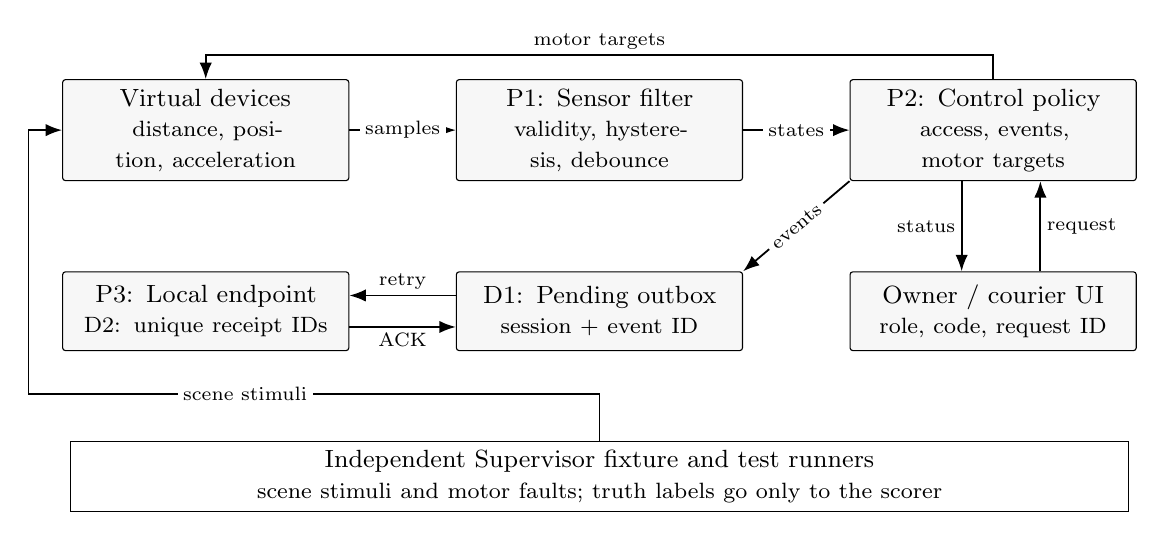
\begin{tikzpicture}[x=1cm,y=1cm,>=Latex,font=\small,
box/.style={draw,rounded corners=1pt,align=center,minimum height=1cm,text width=3.4cm,fill=black!3},
arr/.style={->,line width=.65pt},lab/.style={font=\scriptsize,fill=white,inner sep=2pt}]
\node[box] (devices) at (0,0) {Virtual devices\\\footnotesize distance, position, acceleration};
\node[box] (filter) at (5,0) {P1: Sensor filter\\\footnotesize validity, hysteresis, debounce};
\node[box] (policy) at (10,0) {P2: Control policy\\\footnotesize access, events, motor targets};
\node[box] (endpoint) at (0,-2.3) {P3: Local endpoint\\\footnotesize D2: unique receipt IDs};
\node[box] (queue) at (5,-2.3) {D1: Pending outbox\\\footnotesize session + event ID};
\node[box] (ui) at (10,-2.3) {Owner / courier UI\\\footnotesize role, code, request ID};
\node[draw,align=center,text width=13.2cm,minimum height=.85cm] (fixture) at (5,-4.4) {Independent Supervisor fixture and test runners\\\footnotesize scene stimuli and motor faults; truth labels go only to the scorer};
\draw[arr] (devices)--node[lab]{samples}(filter);
\draw[arr] (filter)--node[lab]{states}(policy);
\draw[arr] (policy.north)--(10,.95)--node[lab,above]{motor targets}(0,.95)--(devices.north);
\draw[arr] (policy.south west)--node[lab,sloped]{events}(queue.north east);
\draw[arr] ([xshift=-.4cm]policy.south)--node[lab,left]{status}([xshift=-.4cm]ui.north);
\draw[arr] ([xshift=.6cm]ui.north)--node[lab,right]{request}([xshift=.6cm]policy.south);
\draw[arr] ([yshift=.2cm]queue.west)--node[lab,above]{retry}([yshift=.2cm]endpoint.east);
\draw[arr] ([yshift=-.2cm]endpoint.east)--node[lab,below]{ACK}([yshift=-.2cm]queue.west);
\draw[arr] (fixture.north) -- (5,-3.35) -- (-2.25,-3.35) -- (-2.25,0) -- (devices.west);
\node[lab] at (.5,-3.35) {scene stimuli};
\end{tikzpicture}
\caption{Data-flow diagram. The fixture changes the scene, while the ordinary Robot reads devices. Trial labels are never an input to the detector. P denotes a process and D an in-memory data store.}\label{fig:dfd}
\end{figure*}

The Robot Window accepts a role, code, and fresh request ID. It displays parcel state, door and bolt feedback, fault reason, and delivery state separately. Scenario controls for parcel placement, impacts, or motor faults are explicitly test controls. They belong to the trusted classroom environment and are not a deployed authentication boundary.

The fixture receives scene commands on channel~3 and event packets on channel~4. It acknowledges received event IDs on channel~1; status observers use channel~2. The ordinary controller cannot query Supervisor scene coordinates. Ground-truth labels remain in the test runners, which compare expected outcomes with emitted events.

\subsection{Mechanical Model and Actuator Feedback}
The enclosure has a hinged door and a linear bolt carried by the door. The bolt's SliderJoint is nested within the door Solid so its position and orientation follow door motion. The test suite observes both bodies while the door is open to verify this attachment. A prior model placed the bolt at the enclosure level, which allowed it to remain suspended in the opening; correcting the hierarchy required rerunning the physical tests and recordings.

Motor commands and measured positions remain distinct. The hinge's physical stops extend slightly beyond the commanded range, preventing the closed target from fighting a coincident hard stop. The bolt has physical travel stops beyond its commanded endpoints. Its fault fixture disables motor force and applies a brake to resist passive motion from the door; the door fixture disables torque. These mechanisms supply repeatable failure injection. This model evaluates sequencing and feedback; it does not model the strength of a real strike plate, forced entry, or safe human handling.

\subsection{Event Transport and Storage}
Each event contains a session namespace, monotonic integer ID, simulation timestamp, kind, and reason. Sensor-derived events also retain the sampled-event timestamp and local queue latency. Entered PINs are omitted from the event export. Pending events remain in memory until an acknowledgment matches both the current session and a pending ID.

The adapter retries batches of up to 16 events every $0.25$ simulated seconds. The endpoint stores each session-qualified ID once and acknowledges repeated packets without processing the event again. Thus packet duplication is allowed while duplicate endpoint processing is rejected. The JSONL log supports inspection, but the controller does not replay it on restart: the outbox, used-code state, and replay cache are volatile.

\section{Control Design and Implementation}
\label{sec:control}
\subsection{Sensor Interpretation}
The distance sensors form a $5\times5$ grid at coordinates $-0.22$, $-0.11$, $0$, $0.11$, and $0.22\,\mathrm{m}$ on each horizontal axis. Each ray uses $0.5\%$ relative Gaussian noise. Let $d_t$ be the minimum valid ray reading at time step $t$. The candidate presence state uses hysteresis:
\begin{equation}
q_t=\begin{cases}
1,&d_t<0.40\,\mathrm{m},\\
0,&d_t\geq0.43\,\mathrm{m},\\
p_{t-1},&\text{otherwise},
\end{cases}
\label{eq:presence}
\end{equation}
where $p_{t-1}$ is the last confirmed presence state. Three consecutive candidate samples confirm a transition. Startup and recovery after invalid data also require three usable samples; an invalid sample resets the debounce count. This avoids inventing a parcel edge across a sensor gap.

The door is closed below $0.05\,\mathrm{rad}$ and open above $0.15\,\mathrm{rad}$. The bolt is retracted at or below $0.006\,\mathrm{m}$ and locked at or above $0.074\,\mathrm{m}$. Intermediate travel cannot authorize opening. Non-finite feedback disables access, ends an active grant, and reports a sensor fault. Unavailable measurements encode as JSON \code{null}, allowing the interface to show the failure without failing to parse status.

\subsection{Access Policy and Motion Sequence}
Courier code \code{2468} expires after 300 simulated seconds and is consumed when access is granted. Owner code \code{1357} also works once and expires after 86,400 seconds. Both tokens are consumed on grant. Each independent motor-cycle trial starts a fresh policy session. Requests are checked for role, expiry, prior use, replay ID, cooldown, occupancy, and a secure starting state. Expiry has an exclusive upper bound: a request at the deadline is rejected. Five failed credential attempts within 300 seconds pause entry for 60 seconds. These fixed codes are simulation fixtures, not production credential management.

Figure~\ref{fig:states} summarizes the normal motion sequence. A successful request retracts the bolt. The door opens only after measured retraction and valid feedback. Closing or reaching the 20-second access deadline immediately revokes the grant; the bolt stays retracted until the door is measured closed. Security status is the conjunction
\begin{equation}
\begin{aligned}
\mathrm{secured}={}&\mathrm{valid}\land\mathrm{closed}\land\mathrm{locked}\\
&\land\neg\mathrm{fault}\land\neg\mathrm{grant}\land\neg\mathrm{closing}.
\end{aligned}
\label{eq:secure}
\end{equation}
A command to extend the bolt cannot satisfy this condition by itself.
\begin{figure*}[t]
\centering
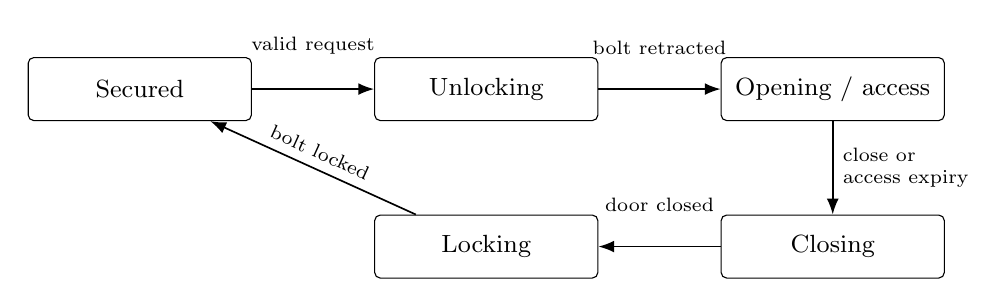
\begin{tikzpicture}[>=Latex,font=\small,statebox/.style={draw,rounded corners=2pt,text width=2.6cm,align=center,minimum height=.8cm},arr/.style={->,line width=.6pt}]
\node[statebox] (s) at (0,0) {Secured};
\node[statebox] (u) at (4.4,0) {Unlocking};
\node[statebox] (a) at (8.8,0) {Opening / access};
\node[statebox] (c) at (8.8,-2) {Closing};
\node[statebox] (l) at (4.4,-2) {Locking};
\draw[arr] (s)--node[above=9pt,font=\scriptsize]{valid request}(u);
\draw[arr] (u)--node[above=9pt,font=\scriptsize]{bolt retracted}(a);
\draw[arr] (a)--node[right,font=\scriptsize,align=left]{close or\\access expiry}(c);
\draw[arr] (c)--node[above=9pt,font=\scriptsize]{door closed}(l);
\draw[arr] (l)--node[above,sloped,font=\scriptsize]{bolt locked}(s);
\end{tikzpicture}
\caption{Normal actuator sequence. Invalid feedback or a motion timeout produces a fault; recovery requires measured feedback, not a new command alone.}\label{fig:states}
\end{figure*}

The bolt has a two-second target timeout. A closing door has three seconds before a door fault. A fault remains visible until the corresponding measured condition recovers. A redundant close command on an already secured box does not renew the impact grace period, so repeated close requests cannot suppress later impacts.

\subsection{Event Rules}
An empty-to-present transition during courier-authorized open-door handling records a parcel-detected event and marks delivery pending. Delivery is recorded only after the parcel remains present, the door is measured closed, the bolt is measured locked, and no grant or fault remains. A blocked bolt leaves delivery pending; parcel removal or suspected tampering cancels it. A present-to-empty transition during owner access creates retrieval. An unexplained opening or parcel transition creates tamper. Outside approved handling and settling, a measured acceleration-axis magnitude above $13\,\mathrm{m/s^2}$ also creates tamper. A one-second refractory interval limits repeated impact alerts, and closure has a $0.7$-second settling grace period. A sequence with no delivery, retrieval, or tamper event is scored as benign motion.

These rules have a deliberate limit: an impact during approved handling can be suppressed with legitimate door motion. The tests establish behavior for the defined scenarios, not recognition of every possible attack. Plausible stuck-at sensor readings also require additional diagnostics beyond non-finite-value detection.

\section{Evaluation Method}
\label{sec:method}
\subsection{Requirements and Acceptance Criteria}
The software requirements document assigns R1--R14 to the numerical targets and delivery obligations. Table~\ref{tab:requirements} connects each requirement to its acceptance evidence. Policy regressions and edge cases run separately from the acceptance experiments and do not add to their trial counts.
\begin{table*}[t]
\centering\small
\caption{Requirements and their acceptance evidence.}\label{tab:requirements}
\begin{tabularx}{\textwidth}{@{}lp{.42\textwidth}Y@{}}
\toprule ID & Acceptance criterion & Evaluation or deliverable \\\midrule
R1 & At least 48 correct presence decisions of 50. & 25 empty and 25 occupied scenes; varied parcel dimensions and positions, including edge placements.\\
R2 & Four-class macro F1 at least 0.90. & 15 final sequences each of benign motion, delivery, retrieval, and tamper.\\
R3 & At most 2 false tamper alarms of 45. & All non-tamper final sequences form the denominator.\\
R4 & At least 99 successful cycles of 100. & Measured full opening, closure, and bolt endpoints.\\
R5 & At least 29 of 30 alerts queued within 1 s. & First sampled impact crossing to local queue insertion, in simulated time.\\
R6 & Recover all 100 offline alerts once. & 10 outages of 10 impacts; compare sender and receiver event IDs.\\
R7 & Zero unauthorized unlocks in 30 attempts. & Six each: invalid, expired, reused, wrong-role, and replayed-ID requests.\\
R8 & Detect blocked bolt motion without false secured status. & Disable force and apply a brake in both directions; release and observe recovery.\\
R9 & Five credential failures trigger a 60 s pause. & Valid code rejected during cooldown and accepted afterward.\\
R10 & Local entry, measured status, history, and fixture controls. & Robot Window and 14 DOM checks, plus layout review.\\
R11 & Repeatable evaluation with saved failure details. & Fixed seeds, separate development/final runs, source/report hashes, JSON/CSV records.\\
R12 & Complete project and communication materials. & Source, paper, presentation with notes, captioned demos, guides, and portable archive.\\
R13 & Record delivery only after measured closure and locking. & Pending, blocked-lock recovery, removal, and offline workflow tests.\\
R14 & Reset safely and resume local operation. & Open-door reset: no grant survives; bolt remains retracted until closure.\\
\bottomrule
\end{tabularx}
\end{table*}

\subsection{Experimental Configuration}
Evaluation uses Webots R2025a, a $32\,\mathrm{ms}$ timestep, and physics seed 42. Development event scenarios use seed 5650. Final event scenarios use seed 20260930; presence trials use seed 20260931. Thresholds and timing are stored in \code{config/evaluation.json}. The evaluation script hashes source, configuration, generated worlds, test code, and UI files before and after execution, then hashes the reports. A change during evaluation causes the run to fail.

Development and final seeds produce different realizations of the same scenario families, not an independent real-world dataset. Configuration is fixed for the final run. The fixture supplies labels only to the scorer; the controller receives sensor measurements and user requests. Each test exports its observations, and any failed acceptance gate causes a nonzero exit status. Results are available with the source release \cite{repository}.

\subsection{Scoring and Timing Definitions}
For class $k$, precision and recall are combined as
\begin{equation}
\begin{aligned}
F_{1,k}&=\frac{2TP_k}{2TP_k+FP_k+FN_k},\\
F_{1,\mathrm{macro}}&=\frac{1}{4}\sum_{k=1}^{4}F_{1,k}.
\end{aligned}
\end{equation}
Rows of the confusion matrix are expected labels and columns are predictions. A sequence containing a tamper event is scored as tamper before delivery or retrieval is considered. The motion-only reference predicts tamper if acceleration exceeds $10.2\,\mathrm{m/s^2}$ or door angle varies by more than $0.05\,\mathrm{rad}$. It has no role or parcel input and cannot predict the two handling classes.

Local queue latency is
\begin{equation}
L_q=t_{\mathrm{insert}}-t_{\mathrm{first\ sampled\ crossing}}.
\end{equation}
It excludes the time before a device first samples the stimulus, transport to the endpoint, interface rendering, and wall-clock execution. The implementation inserts the event synchronously in the same control tick, so a measured $L_q=0$ does not mean instantaneous physical detection. A second measurement spans fixture stimulus to independent observer receipt and exposes the larger interval.

\section{Results and Discussion}
\label{sec:results}
\subsection{Presence, Event Detection, and Motor Operation}
Table~\ref{tab:results} summarizes the final acceptance experiments. The presence detector made \Presence\ correct decisions. All four classes were separated in the 60 generated event sequences, yielding macro F1 \MacroF\ and \FalseAlarms\ false tamper alarms among 45 non-tamper sequences. Table~\ref{tab:confusion} retains the class counts so the aggregate score can be checked directly.
\begin{table}[htbp]\centering\small
\caption{Final evaluation results. All durations refer to simulated time.}\label{tab:results}
\begin{tabularx}{\columnwidth}{@{}Yrr@{}}\toprule
Measure & Observed & Acceptance \\\midrule
Presence decisions & \Presence & $\geq48/50$\\
Four-class macro F1 & \MacroF & $\geq0.90$\\
Non-tamper false alarms & \FalseAlarms/45 & $\leq2/45$\\
Completed motor cycles & \Cycles/100 & $\geq99/100$\\
Alerts queued within 1 s & \LatencyCount/30 & $\geq29/30$\\
Recovered offline alert IDs & \Recovered/100 & $100/100$\\
Unauthorized unlocks & \Unauthorized/30 & $0/30$\\\bottomrule
\end{tabularx}
\end{table}
\begin{table}[htbp]\centering\small
\setlength{\tabcolsep}{3pt}
\caption{Final confusion matrix. Rows are expected labels; columns are predictions.}\label{tab:confusion}
\begin{tabular}{@{}lrrrr@{}}\toprule
 & Benign & Delivery & Retrieval & Tamper\\\midrule
% BEGIN CONFUSION MATRIX
Benign motion & 15 & 0 & 0 & 0\\
Delivery & 0 & 15 & 0 & 0\\
Retrieval & 0 & 0 & 15 & 0\\
Tamper & 0 & 0 & 0 & 15\\
% END CONFUSION MATRIX
\bottomrule\end{tabular}
\end{table}

The motion-only reference achieved macro F1 \BaselineF\ and raised tamper alarms in all 45 non-tamper sequences. This result is consistent with its limited inputs: legitimate handling moves the door, and the alarm cannot use authorization to distinguish it from an unexplained opening. Its score demonstrates the weakness of this particular alarm rule on this suite; it does not establish superiority over tuned or learned alternatives.

All \Cycles\ complete motor cycles reached the required measured endpoints. Jam tests exercised extension and retraction faults separately. The interface remained unsecured during blocked motion, then recovered only when feedback reached the target. A separate door obstruction test kept the bolt retracted while the door remained open. The attachment check additionally verifies that the modeled bolt travels with the open door.

\subsection{Timing, Message Recovery, and Access Checks}
All \LatencyCount\ timing trials inserted an alert within one simulated second of the first sampled threshold crossing. Local queue latency was zero at the control tick's resolution. The maximum measured stimulus-to-observer interval was \ObserverDelay\ seconds. These are local simulation measurements, not network round-trip or phone-notification latencies.

Each of 10 outages generated 10 expected impact events. All \Recovered\ event IDs remained pending offline and were processed once after reconnection. Lost-ACK tests caused retransmission, confirmed duplicate packets at the endpoint, and checked that the unique receipt list remained unique. This demonstrates retry and deduplication while processes remain running; it does not demonstrate crash-safe durability.

The access suite produced \Unauthorized\ unauthorized unlocks in 30 attempts, covering invalid, expired, reused, wrong-role, and replayed-ID requests. Additional checks confirmed that a valid code is rejected during cooldown and succeeds after the pause. Automatic access expiry also returned the enclosure to a measured secure state.

\subsection{Failures Found and Corrected}
The development record includes an intentionally failed hinge-contact experiment. Coincident hard stops and the commanded closed position caused contact forces that appeared as false impact alarms. The final model separates the hard-stop range from the normal motor target and retains the failed diagnostic for comparison. The failed file is excluded from acceptance evidence rather than relabeled as a passing result.

The proposal audit corrected delivery recording before latch confirmation and made the owner temporary code single-use. Added cases verify pending delivery during a blocked lock, cancellation after removal, a complete offline delivery and retrieval, and safe reset with the door open.

Review also found that redundant close requests could renew the impact grace period, that non-finite readings required safe JSON encoding, and that sensor gaps needed to reset consecutive-sample counts. Regression cases now exercise those paths. The final physical review corrected the bolt's parent body, added physical slider stops and a brake for fault injection, and repeated the evaluation because changing the mechanism changes its dynamics. The \Regressions\ policy checks and simulator edge cases test these corrections separately from the acceptance trials.

\section{Conclusions and Future Work}
\label{sec:conclusion}
Parcel Guard met each numerical target in the proposal on the generated Webots trials. The controller records delivery after the door closes and the bolt locks, keeps local access working during link outages, and reports blocked motion as a fault. The saved trial records and source allow these results to be repeated.

The evaluation has several limits. Parcel placement is scripted rather than performed by a modeled courier hand. The physical model does not establish lock strength, weather resistance, pinch safety, or forced-entry protection. The simulated link does not model TLS, radio propagation, or an external notification provider. Fixed demo credentials and exposed fixture controls are unsuitable for deployment. Event storage and credential-use state disappear on restart, and plausible stuck sensors can evade validity checks. The test set is small and generated from known scenario families; perfect classification here should not be extrapolated to field behavior.

The next implementation priorities follow those limits: persist the outbox and credential state with recovery tests; separate authenticated operational commands from fixture control; add plausibility and stuck-sensor diagnostics; and test measured hardware traces before changing classification thresholds. A physical prototype would also require a strike mechanism, safe motion limits, enclosure testing, and trials with varied parcels and handling. These extensions would need their own acceptance tests.

\balance
\appendices
\section{Reproduction and Submission Guide}
\label{sec:reproduce}
The complete archive includes generated worlds, Python modules, the local interface, test runners, saved JSON/CSV results, raw recordings, final videos, this report's editable LaTeX source, and presentation slides with speaker notes. To run the project and check the saved results:
\begin{enumerate}
\item Extract the archive. Run \code{python3 scripts/\allowbreak check\_submission.py} to verify included files and saved evidence hashes without optional document or video packages.
\item Install Webots R2025a and Python 3.10 or newer. Open \code{worlds/delivery\_box.wbt}. The local Robot Window exposes owner/courier entry and separate scenario controls.
\item Run \code{python3 scripts/\allowbreak run\_all.py} to regenerate worlds and repeat the policy and simulator evaluation. Set \code{WEBOTS\_BIN} if the executable is not discoverable.
\item Inspect \code{results/REPORT.md}, the JSON reports, and the evaluation manifest. The manifest records runtime versions, source hashes, and report hashes.
\end{enumerate}

The report source is \code{docs/\allowbreak parcel\_guard\_report.tex}. It is a standalone LaTeX file with embedded vector diagrams. The report build script refreshes evidence values from passing reports and exports the PDF. The presentation guide maps the 14-slide deck to the proposal slides' suggested 13-minute talk and two-minute question period. The final walkthrough is captioned without narration; the two shorter clips support in-class playback. The project archive is version \ReportVersion. Submission requires uploading the requested PDF and presenting the work in class.

\begin{thebibliography}{9}
\bibitem{amazon} S. Wolfson, ``What is Amazon Key In-Garage Delivery?,'' Amazon, updated September 28, 2023. \url{https://www.aboutamazon.com/news/amazon-prime/what-is-amazon-key-in-garage-delivery}.
\bibitem{yale} Yale, \emph{Yale Smart Security Box: User Manual}. \url{https://www.yalehome.com/apac-blueprint/en/images/product-assets/safe/yale-smart-security-box/assets/documents/user-manual/user-manual-yale-smart-security-box.pdf}.
\bibitem{distance} Cyberbotics, ``DistanceSensor,'' \emph{Webots Reference Manual}, R2025a. \url{https://github.com/cyberbotics/webots/blob/R2025a/docs/reference/distancesensor.md}.
\bibitem{position} Cyberbotics, ``PositionSensor,'' \emph{Webots Reference Manual}, R2025a. \url{https://github.com/cyberbotics/webots/blob/R2025a/docs/reference/positionsensor.md}.
\bibitem{acceleration} Cyberbotics, ``Accelerometer,'' \emph{Webots Reference Manual}, R2025a. \url{https://github.com/cyberbotics/webots/blob/R2025a/docs/reference/accelerometer.md}.
\bibitem{supervisor} Cyberbotics, ``Supervisor Programming,'' \emph{Webots User Guide}, R2025a. \url{https://github.com/cyberbotics/webots/blob/R2025a/docs/guide/supervisor-programming.md}.
\bibitem{proposal} J. Guico, J. Jimenez, and B. Lopez, \emph{Package Delivery Security Box: Webots Simulation for Secure Package Delivery}, CS 5650 project proposal, California State University, Los Angeles, Sept. 2026.
\bibitem{rubric} CS 5650 course materials, \emph{Final Report Guidelines and Format Recommendation}; final-exam task description; and software-engineering design, implementation, evaluation, oral and written communication rubric. Supplied assignment screenshots.
\bibitem{repository} J. Guico, J. Jimenez, and B. Lopez, \emph{Parcel Guard Webots Project}, version \ReportVersion, source and evaluation evidence. \url{https://github.com/joejimenez-lab/parcel-guard-webots}.
\end{thebibliography}
\end{document}
